\documentclass{ximera}

\input{../preamble.tex}




\title{Derivatives of inverse trigonometric functions}

\begin{document}
\begin{abstract}
  We derive the derivatives of inverse trigonometric functions using implicit
  differentiation.
\end{abstract}
\maketitle

Now we will derive the derivative of arcsine, arctangent, and
arcsecant.

%% Since this is an inverse
%% function, we can find its derivative by using implicit
%% differentiation and the Inverse Function Theorem.


\begin{theorem}[The derivative of arcsine]\index{derivative!of arcsine}
\[
\frac{d}{dx} \arcsin(x) = \frac{1}{\sqrt{1-x^2}}.
\]
\begin{explanation} 
  %% To start, note that the Inverse Function Theorem assures us that this
  %% derivative actually exists.
  If $y=\arcsin(x)$ then $\sin(y) = x$ and $\answer[given]{\frac{-\pi}{2}}\le
  y\le \answer[given]{\frac{\pi}{2}}$.
  Implicitly differentiating with respect $x$ we see
  \begin{align*}
    \sin(y) &= x\\
    \frac{d}{dx} \sin(y) &= \frac{d}{dx} x &\text{Differentiate both sides.}\\
    \cos(y) \cdot \frac{dy}{dx} &= 1 &\text{Implicit differentiation.}\\
    \frac{dy}{dx} &= \frac{1}{\cos(y)} &\text{Solve for $\frac{dy}{dx}$.}
  \end{align*}
  While $\frac{dy}{dx} = \frac{1}{\cos(y)}$, we need our final answer for $\frac{dy}{dx}$ written
  in terms of $x$. Since we are assuming that
  \[
  \sin(y) =\mbox{opp/hyp}= x=x/1,
  \]
  we can draw the right triangle below:
      \begin{image}[2in]
      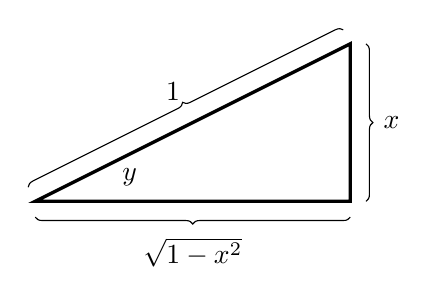
\begin{tikzpicture}
        \coordinate (C) at (0,2);
        \coordinate (D) at (4,2);
        \coordinate (E) at (4,4);
        \tkzMarkRightAngle(C,D,E)
        \tkzMarkAngle(D,C,E)
        \draw[decoration={brace,mirror,raise=.2cm},decorate,thin] (0,2)--(4,2);
        \draw[decoration={brace,mirror,raise=.2cm},decorate,thin] (4,2)--(4,4);
        \draw[decoration={brace,raise=.2cm},decorate,thin] (0,2)--(4,4);
        \draw[very thick] (D)--(E)--(C)--cycle;
        \node at (2,2-.65) {$\sqrt{1-x^2}$};
        \node[anchor=west] at (4+.3,3) {$x$};
        \node at (2-.25,3+.4) {$1$};
        \node at (1.2,2.3) {$y$};
      \end{tikzpicture}
    \end{image}

%  consider the following triangle with the unit circle:
%  \begin{image}
%    \begin{tikzpicture}
%      \begin{axis}[
%          xmin=-1.1,xmax=1.1,ymin=-1.1,ymax=1.1,
%          axis lines=center,
%          width=4in,
%          ticks=none,
%          clip=false,
%          unit vector ratio*=1 1 1,
%          %xlabel=$x$, ylabel=$y$,
%          every axis y label/.style={at=(current axis.above origin),anchor=south},
%          every axis x label/.style={at=(current axis.right of origin),anchor=west},
%        ]        
%        \addplot [penColor2!50!white, very thick, smooth, domain=(-90:90)] ({cos(x)},{sin(x)}); %% unit circle
%        \addplot [black!50!white, dashed, smooth, domain=(90:270)] ({cos(x)},{sin(x)}); %% unit circle
%        \addplot[color=penColor2!50!white,fill=penColor2!50!white,only marks,mark=*] coordinates{(0,1)};  %% closed hole
%        \addplot[color=penColor2!50!white,fill=penColor2!50!white,only marks,mark=*] coordinates{(0,-1)};  %% closed hole         
%        \addplot [ultra thick] plot coordinates {(0,0) (.766,.643)}; %% 40 degrees
%        
%        \addplot [ultra thick] plot coordinates {(.766,0) (.766,.643)}; %% 40 degrees
%        \addplot [ultra thick] plot coordinates {(0,0) (.766,0)}; %% 40 degrees
%        
%        %\addplot [ultra thick,penColor3] plot coordinates {(1,0) (1,.839)}; %% 40 degrees          
%        
%        \addplot [textColor,smooth, domain=(0:40)] ({.15*cos(x)},{.15*sin(x)});
%        %\addplot [very thick,penColor] plot coordinates {(0,0) (.766,.643)}; %% sector
%        %\addplot [very thick,penColor] plot coordinates {(0,0) (1,0)}; %% sector
%        %\addplot [very thick, penColor, smooth, domain=(0:40)] ({cos(x)},{sin(x)}); %% sector
%        \node at (axis cs:.12,.07) [anchor=west] {$\theta$};
%        \node at (axis cs:.84,.322) {$x$};
%        \node at (axis cs:.383,0) [anchor=north] {$\sqrt{1-x^2}$};
%        \node at (axis cs:.38,.32) [anchor=south] {$1$};
%      \end{axis}
%    \end{tikzpicture}
%  \end{image}
  From the image above, we see that 
  \begin{align*}
    \frac{dy}{dx} &= \frac{1}{\cos(y)}\\
    &=\frac{\mathrm{hyp}}{\mathrm{adj}}\\
    &= \answer[given]{\frac{1}{\sqrt{1-x^2}}}.
  \end{align*}
   This formula agrees with the fact that $\cos(y)\ge 0$ on our restricted interval $\Bigl(-\frac{\pi}{2},\frac{\pi}{2}\Bigr)$.\\
   
  In summary,
  \[
  \frac{dy}{dx} = \frac{d}{dx} \arcsin(x) = \answer[given]{\frac{1}{\sqrt{1-x^2}}}.
  \]
 
\end{explanation}
\end{theorem}


\begin{question}
  Compute:
  \[
  \frac{d}{dx} \arcsin(x^3)
  \begin{prompt}
    = \answer[given]{\frac{3x^2}{\sqrt{1-(x^3)^2}}}
  \end{prompt}
  \]
\end{question}



We can do something similar with arctangent. 


\begin{theorem}[The derivative of arctangent]\index{derivative!of arctangent}
  \[
  \frac{d}{dx} \arctan(x) = \frac{1}{1+x^2}.
  \]
  \begin{explanation} 
%     To start, note that the Inverse Function Theorem assures us that this
%     derivative actually exists.
    If
    \(
    \arctan(x) = y
    \)
    then $\tan(y) = x$ and $\answer[given]{\frac{-\pi}{2}}<
    y< \answer[given]{\frac{\pi}{2}}$.  Implicitly
    differentiating with respect $x$ we see
    \begin{align*}
      \tan(y) &= x\\
      \frac{d}{dx} \tan(y) &= \frac{d}{dx} x         &\text{Differentiate both sides.}\\
      \sec^2(y) \cdot \frac{dy}{dx} &= 1   &\text{Implicit differentiation.}\\
     \frac{dy}{dx} &= \frac{1}{\sec^2(y)}   &\text{Solve for $\frac{dy}{dx}$.}
       \end{align*}
      Recall the trig identity:  $\sec^2(y)=1+\tan^2(y)$.\\
        \begin{align*}
          \frac{dy}{dx} &= \frac{1}{1+\tan^2(y)} 
         \end{align*}
         Since  $\tan(y) = x$, we have\\
          \begin{align*}
          \frac{dy}{dx} &= \frac{1}{1+x^2} .
         \end{align*}
         
         Instead of using the Pythagorean identity above, we could also assemble a right triangle using $\tan(y)=x/1$ to arrive at the same final conclusion.
  %%  While $\theta' = \cos^2(\theta)$, we need our answer written in terms
    %of $x$. Since we are assuming that
   % \[
   % \tan(\theta) = \frac{\sin(\theta)}{\cos(\theta)}= x,
   % \]
   % we may consider the following triangle:
    %\begin{image}[2in]
     % \begin{tikzpicture}
      %  \coordinate (A) at (5*.766,5*0);
        %\coordinate (B) at (5*.766,5*.643);
       % \coordinate (C) at (0,0);
       % \tkzMarkRightAngle(C,A,B)
        %\tkzMarkAngle[size=.6cm,thin](A,C,B)
        
	%\draw[very thick] (A)--(B)--(C)--cycle;
        %\node at (5*.10,5*.06) [anchor=west] {$\theta$};
       % \node at (5*.766,5*.322)[anchor=west] {$x$};
       % \node at (5*.383,0) [anchor=north] {$1$};
        %\node at (5*.38,5*.32) [above left] {$\sqrt{1+x^2}$};
   % \end{tikzpicture}
    %\end{image}
    %We may now scale this triangle by a factor of $\frac{1}{\sqrt{1+x^2}}$ to place
   % it on the unit circle:
   % \begin{image}
      %\begin{tikzpicture}
	%\begin{axis}[
           % xmin=-1.1,xmax=1.1,ymin=-1.1,ymax=1.1,
            %axis lines=center,
            %width=4in,
            %ticks=none,
           % clip=false,
           % unit vector ratio*=1 1 1,
            %xlabel=$x$, ylabel=$y$,
           % every axis y label/.style={at=(current axis.above origin),anchor=south},
           % every axis x label/.style={at=(current axis.right of origin),anchor=west},
        %  ]        
         % \addplot [penColor3!50!white, very thick, smooth, domain=(-90:90)] ({cos(x)},{sin(x)}); %% unit circle
          %\addplot [black!50!white, dashed, smooth, domain=(90:270)] ({cos(x)},{sin(x)}); %% unit circle
          %\addplot[color=penColor3!50!white,fill=white,only marks,mark=*] coordinates{(0,1)};  %% open hole
          %\addplot[color=penColor3!50!white,fill=white,only marks,mark=*] coordinates{(0,-1)};  %% open hole     
          %\addplot [ultra thick] plot coordinates {(0,0) (.766,.643)}; %% 40 degrees

         % \addplot [ultra thick] plot coordinates {(.766,0) (.766,.643)}; %% 40 degrees
         % \addplot [ultra thick] plot coordinates {(0,0) (.766,0)}; %% 40 degrees
          
          %\addplot [ultra thick,penColor3] plot coordinates {(1,0) (1,.839)}; %% 40 degrees          

         % \addplot [textColor,smooth, domain=(0:40)] ({.15*cos(x)},{.15*sin(x)});
          %\addplot [very thick,penColor] plot coordinates {(0,0) (.766,.643)}; %% sector
          %\addplot [very thick,penColor] plot coordinates {(0,0) (1,0)}; %% sector
          %\addplot [very thick, penColor, smooth, domain=(0:40)] ({cos(x)},{sin(x)}); %% sector
         % \node at (axis cs:.12,.07) [anchor=west] {$\theta$};
         % \node at (axis cs:.84,.322)[anchor=west] {$\frac{x}{\sqrt{1+x^2}}$};
         % \node at (axis cs:.383,0) [anchor=north] {$\frac{1}{\sqrt{1+x^2}}$};
          %\node at (axis cs:.38,.32) [anchor=south] {$1$};
        %\end{axis}
%\end{tikzpicture}
%\end{image}
%%From the unit circle above, we see that 
%%\begin{align*}
%%  \theta' &= \cos^2(\theta)\\
 %% &= \left(\frac{\mathrm{adj}}{\mathrm{hyp}}\right)^2\\
  %&= \answer[given]{\frac{1}{1+x^2}}.
%%\end{align*}
In summary,
\[
\frac{dy}{dx} = \frac{d}{dx} \arctan(x) = \answer[given]{\frac{1}{1+x^2}}.
\]
\end{explanation}
\end{theorem}

\begin{question}
  Compute:
  \[
  \frac{d}{dx} \tan^{-1}(\sqrt{x})
  \begin{prompt}
    = \answer[given]{\frac{1}{1+(\sqrt{x})^2}\cdot\frac{1}{2\sqrt{x}}}
  \end{prompt}
  \]
\end{question}



Finally, we investigate the derivative of arcsecant.

\begin{theorem}[The derivative of arcsecant]\index{derivative!of arcsecant}
\[
\frac{d}{dx} \arcsec(x) = \frac{1}{|x|\sqrt{x^2-1}}\qquad\text{for $|x|>1$.}
\]
\begin{explanation} 
  %% To start, note that the Inverse Function Theorem assures us that this
  %% derivative actually exists.
  If
\(
\arcsec(x) = y
\)
then $\sec(y) = x$ and $\answer[given]{0}\le y\le
\answer[given]{\pi}$ with $\theta\ne \answer[given]{\pi/2}$.  Implicitly
differentiating with respect $x$ we see
\begin{align*}
\sec(y) &= x\\
\frac{d}{dx} \sec(y) &= \frac{d}{dx} x                     &\text{Differentiate both sides.}\\
\sec(y)\tan(y) \cdot \frac{dy}{dx} &= 1     &\text{Implicit differentiation.}\\
\frac{dy}{dx} &= \frac{1}{\sec(y)\tan(y)}=\frac{\cos^2(y)}{\sin(y)} &\text{Solve for $\frac{dy}{dx}$}.
\end{align*}
While $\frac{dy}{dx} = \frac{\cos^2(y)}{\sin(y)}$, we need our final
answer written in terms of $x$. Since we are assuming that
\[
\sec(y) = \frac{1}{\cos(y)}= x,
\]
we have $\cos(y)=1/x=$adj/hyp and we assemble the following right triangle:
    \begin{image}[2in]
      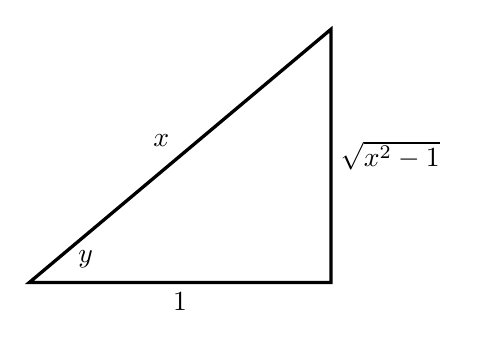
\begin{tikzpicture}
        \coordinate (A) at (5*.766,5*0);
        \coordinate (B) at (5*.766,5*.643);
        \coordinate (C) at (0,0);
        \tkzMarkRightAngle(C,A,B)
        \tkzMarkAngle[size=.6cm,thin](A,C,B)
        
	\draw[very thick] (A)--(B)--(C)--cycle;
        \node at (5*.10,5*.06) [anchor=west] {$y$};
        \node at (5*.766,5*.322)[anchor=west] {$\sqrt{x^2-1}$};
        \node at (5*.383,0) [anchor=north] {$1$};
        \node at (5*.38,5*.32) [above left] {$x$};
    \end{tikzpicture}
    \end{image}
    
    And thus
%    We may now scale this triangle by a factor of $\frac{1}{x}$ to place
%    it on the unit circle:
%\begin{image}
%\begin{tikzpicture}
%	\begin{axis}[
%            xmin=-1.1,xmax=1.1,ymin=-1.1,ymax=1.1,
%            axis lines=center,
%            width=4in,
%            ticks=none,
%            clip=false,
%            unit vector ratio*=1 1 1,
%            %xlabel=$x$, ylabel=$y$,
%            every axis y label/.style={at=(current axis.above origin),anchor=south},
%            every axis x label/.style={at=(current axis.right of origin),anchor=west},
%          ]        
%          \addplot [penColor4!50!white, very thick, smooth, domain=(0:180)] ({cos(x)},{sin(x)}); %% unit circle
%          \addplot [black!50!white, dashed, smooth, domain=(180:360)] ({cos(x)},{sin(x)}); %% unit circle
%          \addplot[color=penColor4!50!white,fill=white,only marks,mark=*] coordinates{(0,1)};  %% open hole
%          \addplot[color=penColor4!50!white,fill=penColor4!50!white,only marks,mark=*] coordinates{(1,0)};  %% closed hole
%          \addplot[color=penColor4!50!white,fill=penColor4!50!white,only marks,mark=*] coordinates{(-1,0)};  %% closed hole     
%          \addplot [ultra thick] plot coordinates {(0,0) (.766,.643)}; %% 40 degrees
%
%          \addplot [ultra thick] plot coordinates {(.766,0) (.766,.643)}; %% 40 degrees
%          \addplot [ultra thick] plot coordinates {(0,0) (.766,0)}; %% 40 degrees
%          
%          %\addplot [ultra thick,penColor3] plot coordinates {(1,0) (1,.839)}; %% 40 degrees          
%
%          \addplot [textColor,smooth, domain=(0:40)] ({.15*cos(x)},{.15*sin(x)});
%          %\addplot [very thick,penColor] plot coordinates {(0,0) (.766,.643)}; %% sector
%          %\addplot [very thick,penColor] plot coordinates {(0,0) (1,0)}; %% sector
%          %\addplot [very thick, penColor, smooth, domain=(0:40)] ({cos(x)},{sin(x)}); %% sector
%          \node at (axis cs:.12,.07) [anchor=west] {$\theta$};
%          \node at (axis cs:.84,.322)[anchor=west] {$\sqrt{1-\frac{1}{x^2}}$};
%          \node at (axis cs:.383,0) [anchor=north] {$\frac{1}{x}$};
%          \node at (axis cs:.38,.32) [anchor=south] {$1$};
%        \end{axis}
%\end{tikzpicture}
%\end{image}
%From the unit circle above, we see that 
\begin{align*}
\frac{dy}{dx}&= \frac{\cos^2(y)}{\sin(y)}\\
  &= \frac{
    \left(\frac{\mathrm{adj}}{\mathrm{hyp}}\right)^2}{\frac{\mathrm{opp}}{\mathrm{hyp}}}\\
  &= \frac{\answer[given]{1/x^2}}{\sqrt{1-1/x^2}}&\text{Factoring $1/x^2$ out of the root,}\\
  &= \frac{1}{|x|\sqrt{x^2-1}},
\end{align*}
In summary,
\[
\frac{dy}{dx}= \frac{d}{dx} \arcsec(x) = \frac{1}{|x|\sqrt{x^2-1}}\qquad\text{for $|x|>1$}. 
\]
\end{explanation}
\end{theorem}

\begin{question}
  Compute:
  \[
  \frac{d}{dx} \sec^{-1}(3x)
  \begin{prompt}
    = \answer[given]{\frac{3}{|3x|\sqrt{(3x)^2-1}}}
  \end{prompt}
  \]
\end{question}

We leave it to you, the reader, to derive in a similar fashion the derivatives of
cosine, arccosecant, and arccotangent, listed below.

\begin{theorem}[The Derivatives of Inverse Trigonometric Functions] \hfil
\begin{itemize}
\item $\frac{d}{dx} \arcsin(x) = \frac{1}{\sqrt{1-x^2}}$
\item $\frac{d}{dx} \arccos(x) = \frac{-1}{\sqrt{1-x^2}}$
\item $\frac{d}{dx} \arctan(x) = \frac{1}{1+x^2}$
\item $\frac{d}{dx} \arcsec(x) = \frac{1}{|x|\sqrt{x^2-1}}$ for $|x|>1$
\item $\frac{d}{dx} \arccsc(x) = \frac{-1}{|x|\sqrt{x^2-1}}$ for $|x|>1$
\item $\frac{d}{dx}  \arccot(x) = \frac{-1}{1+x^2}$
\end{itemize}
\end{theorem}

\subsection{Learning Objectives}
After completing this section, students should be able to:
\vspace{.05in}

\noindent$\bullet$ Derive the derivatives of inverse trig functions.
\\$\bullet$ Know the derivatives of the six inverse trig functions.
\\$\bullet$ Differentiate using the inverse trig derivatives.

%\outcome{Derive the derivatives of inverse trigonometric functions.}
%\outcome{Understand how the derivative of an inverse function relates to the original derivative.}
%\outcome{Take derivatives which involve inverse trigonometric functions.}




\end{document}